\section{Designing a Visualization of Gender Diversity in Tech}\label{sec:design}
Interactive narrative visualizations, then, provide an ideal way to present the state of gender diversity (or lack thereof) in tech. Interactive visualizations let viewers explore the data on gender diversity across the tech education pipeline, which allows for deeper engagement than viewing isolated statistics. The narrative thread provides context to motivate that exploration, while also providing an interpretive guide for viewers who may have limited background knowledge. The remainder of the paper outlines the design and development of a web project to provide this guided exploration of the tech education pipeline. My primary goals for this project are to raise awareness of the state of gender diversity in tech, to encourage familiarity with the most-cited data on diversity, and to provide resources for those who are interested in learning more about why diversity matters and what they can do to help.

The conversation about gender in tech is not new. Academic research in the field is well established. By the mid-2000s, even comprehensive reviews of previous work ignored entire bodies of literature that were thought to be settled \citep{Sanders2005Gender}. Popular media and large tech companies have long identified gender diversity as an area for improvement; the Internet Archive has preserved corporate diversity statements from Google beginning in 2011\footnote{\url{https://web.archive.org/web/20110406064303/http://www.google.com/diversity/index.html}}, from Microsoft in 2012\footnote{\url{https://web.archive.org/web/20121006064818/http://www.microsoft.com/en-us/diversity/}}, and from Apple in 2014\footnote{\url{https://web.archive.org/web/20140812164241/http://www.apple.com/diversity/}}. While parts of tech have become more diverse following these discussions, the improvements are rather modest. Presenting recent data highlights the surprisingly small effect of the diversity conversation on actual diversity statistics, so that viewers realize diversity is in no way a solved problem.

Similarly, by helping users explore full datasets rather than mentioning isolated statistics, I hope to build familiarity with the data behind this ongoing discussion. Even the most commonly cited datasets contain richer information than just the number of girls who study computer science as high schoolers, or the percent of the tech work force that is female. Exposure to the breadth of information available can spark new questions: instead of simply asking ``How many women work in tech?'', we can ask ``Why do more women work in web development than in systems administration?'' Asking better questions is essential to finding better answers.

Finally, the visualization page should direct viewers to external resources that will help them explore the broader conversation about diversity in tech. People can engage with a topic in many different ways, and there should be resources for viewers with any level of background knowledge. Many different kinds of resources are therefore included, such as:
\begin{itemize}
  \item Source data for the visualizations, so that viewers can explore on their own
  \item Corporate diversity policies, to see how tech companies have responded to calls for diversity
  \item Nonprofit and professional organizations, who intervene to introduce women and girls to technology and provide support to keep them there
  \item Media coverage, to showcase how issues of diversity are addressed and discussed within broader tech culture
\end{itemize}

I discuss the design for this webpage in the following sections, including its intended audience (\S\ref{sec:design-users}), the questions it should answer (\S\ref{sec:design-tasks}), the specific design goals for the project (\S\ref{sec:design-goals}), and the data selected to address those goals (\S\ref{sec:design-data}).



\subsection{Users}\label{sec:design-users}
For this project, I used a user-centered design approach, beginning by identifying the characteristics and goals of its target audience. With those users in mind, I determined the tasks the final webpage should support---what kinds of questions it needed to answer, how much context it would provide, and what resources it should include for further exploration. These decisions guided the selection of relevant design principles, which in turn shaped the resulting designs.

My project is intended for a general audience, not simply for women's advocates within technology. Most viewers will probably have an interest in the topic, either as a woman, as someone who cares about technology, or both; but they may not have any exposure to gender diversity statistics within tech. This motivates the narrative thread throughout the page, rather than analytical visualizations presented without comment, both to provide context and to help viewers interpret the data visualizations.

I used two primary personas to guide my design work:
\begin{itemize}
  \item Gabriella Griffin, 19, undergraduate psychology major
  \item Laurie Woods, 28, web designer/front-end developer
\end{itemize}
Together, they include both casual audiences (Gabriella) and those invested in diversity in tech (Laurie). Details for each persona are included in \autoref{fig:personas}.

\begin{figure}
  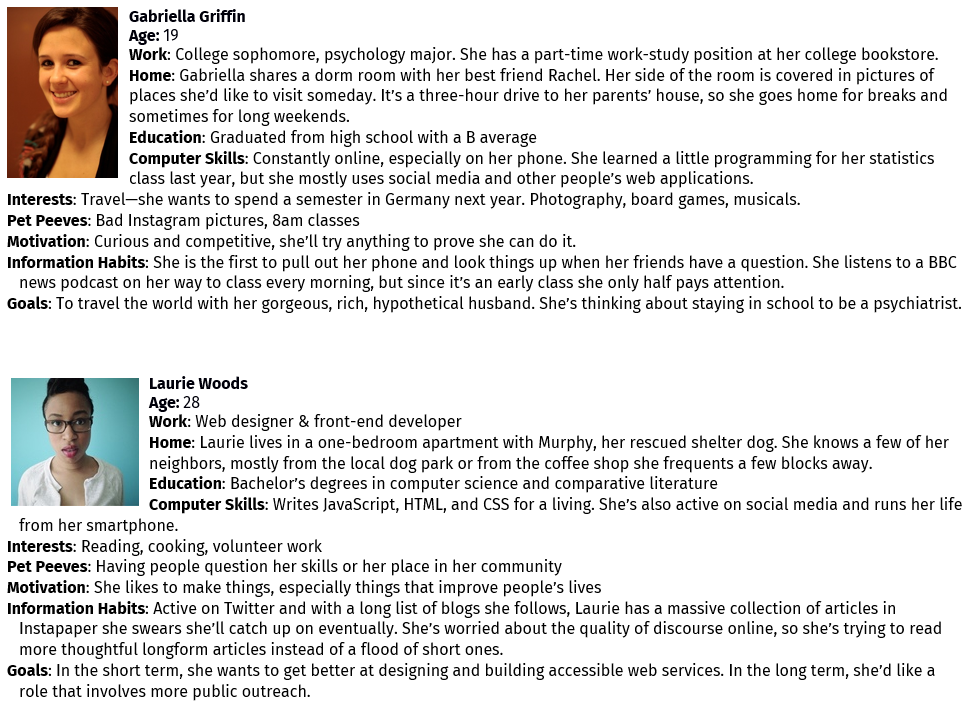
\includegraphics[width=0.95\textwidth]{personas}
  \caption{Primary Personas: Gabriella Griffin \& Laurie Woods}\label{fig:personas}
\end{figure}

\subsection{Tasks}\label{sec:design-tasks}
I do not assume viewers have any prior exposure to diversity statistics or to the tech industry. For users like Gabriella, the primary task the project supports is noticing the gender imbalance at all stages in the tech pipeline. Users like Laurie, who are already aware of the problem, can explore the statistics to see the extent of the problem. The project provides an overview of the data to give this high-level introduction to tech demographics, then presents each stage of the pipeline individually, allowing viewers to explore questions like:

\begin{itemize}
  \item When do women get involved in tech? Is a computer science degree required?
  \item Where does the pipeline leak? Is there a stage when more women seem to drop out?
  \item What kinds of technical careers are open to women? What kinds are still relatively closed?
  \item Does exposing girls to computer science at younger ages lead to more women working in IT\@?
\end{itemize}

The project should also answer questions about the importance of gender diversity in tech and about the interventions used to increase women's participation in IT\@. Some of this will come from the resources list, some from the narration.


\subsection{Design Goals}\label{sec:design-goals}
The webpage's design crucially needs to support exploring these kinds of questions, regardless of technical background or analytical skills. I focused on this need through several specific design goals:
\begin{description}
  \item[Overview first, with details on demand:] Adapted from \citet{Shneiderman1996Eyes}, this mantra of information visualization shaped the narrative structure of the project. Upon loading the webpage, viewers should immediately have an overview of women's participation along the tech education pipeline, with access to more detailed about each stage.
  \item[Consistency:] Detailed views of each stage in the pipeline should be presented consistently, to facilitate comparison of similar information across stages.
  \item[Use simple displays:] Data should be presented in familiar graphs wherever possible, so viewers can explore the data without being distracted by the form of the graph.
  \item[Guide interpretations:] Viewers without much background may have difficulty interpreting data, especially after the first few views. Use the narrative structure to guide viewers easily toward points of interest.
\end{description}


\subsection{Data Selection}\label{sec:design-data}
There are many sources of data on women in computing, from case studies of single computer science departments to occupation data at a national level. For the initial stage of this project, I chose to use publicly available datasets for each stage in the tech education pipeline that (a) include nation-wide data for the United States, (b) are cited in both the academic literature and in media reports, and (c) are structured similarly to aid in comparison across time stages. These criteria led me to three data sources, spanning high school education to industry employment.

\subsubsection*{The College Board's AP Computer Science Test Taker Demographics}
The College Board's Advanced Placement (AP) program offers high school students the opportunity to earn college credit for courses taken in high school by passing standardized exams. Each AP exam covers introductory college-level material within a single subject area. The exams are scored on a 1--5 scale, with scores 3--5 considered passing and eligible for college credit. AP exam data does not include students who are exposed to computing through other means, including the after-school programs that are popular interventions to introduce girls to coding. However, it provides consistent national data on the students who receive a rigorous introduction to computer science while in high school, and it is commonly used as a proxy for computing education before college.

\subsubsection*{The Annual Taulbee Survey of Diversity in Computing Education}
The nonprofit Computing Research Association (CRA) conducts and publishes the Taulbee Survey, an annual report on enrollment in computing programs in higher education. It reports on the number of students and faculty in computer science, computer engineering, and information departments across the United States, and gives demographic breakdowns for each education level. Because this project focuses on the traditional tech pipeline from high school to industry employment, I use the Taulbee data on bachelor's, master's, and PhD degrees awarded and exclude data on faculty and postdoctoral positions.

\subsubsection*{The Bureau of Labor Statistics' Employment Report by Occupation}
The United States Bureau of Labor Statistics posts detailed data by occupation as part of its Current Population Survey, broken down by gender and ethnicity. This includes a fairly granular section of ``Computing Occupations'', including specialties like database administration and web development.

These three sources are ideal for comparison for several reasons. First, they all have a national scope, avoiding the sample size problems of many single-department or regional case studies. Second, they are all regularly cited in existing research on diversity in tech and are publicly available for verification. Finally, they have a similar structure, with breakdowns by gender and by occupational or educational category. This makes them easy to present consistently, while allowing supplementary data to be added in the future to explore facets specific to that stage in the pipeline.
